\chapter{Introduction}
\section{The Smiths}

The Smiths is a startup created in early 2015 in Amsterdam, by two people, Wienke \textsc{Giezeman}, a Dutch entrepreneur, and Pierre \textsc{Van De Velde}, a French developer, who is also a former employee of Wienke.

\subsection{Behind the scenes}

Back in 2012, Wienke created a first startup called WappZapp (a video-on-demand service provider for the Dutch public). He hired Pierre as an intern, in 2013.

\medskip

During 2014, while unceasingly growing at a regular pace, they changed their economic model, offering customers more services (basically, more content to watch) for a few euros. Then, they had been struggling for months, trying to convert all the users to that new freenium model, without success. Although the product was quite robust and this pricing strategy was supposed to work, it is always hard to convince customers, especially those used to free mobile apps. At this point, they just decided to stop there.

\medskip

Soon after, Wienke and Pierre got back to work, both of them owning their own little company (self-employment). Pierre had gained experience with Titanium, a cross-platform SDK\footnote{\textit{Software Development Kit}, a set of software development tools allowing the creation of applications (from software programs to hardware frameworks, video-games, and so on).} for mobile development, as it was the one they used for WappZapp. Quite naturally, they continued working with it: developing apps with Titanium for clients (companies or individuals), that is what they decided to do for a living. Wienke would be the CEO and responsible for finding clients whereas Pierre would be the CTO and developer. A few weeks later they were hiring Matthias as an intern. In solely a couple of weeks, \textbf{from the ashes of WappZapp was born The Smiths}.

\subsection{Who \& What}

At the moment, The Smiths is a sort of agency, "\textit{supplying companies with Titanium developers}" (that is their motto), with full expertise in mobile applications developed with Titanium.

\medskip

As I wrote above, in February 2015, they hired Matthias \textsc{Benkort}, a French student in Computer Science, as an intern. Six months later, he graduated. Then, they decided to offer him a full-time position, which he accepted. That happened approximately when I arrived, in late September 2015. Since the very beginning, they have also been working closely with a Dutch independent designer, still a student but also a freelancer in his spare time, Wessel \textsc{Versluis}. In the meantime, they also hired a remote developer from Vietnam, Nguyen \textsc{Bao Duy}, a freelancer, who would be working from time to time for the company.

\medskip

The goal of the company is pretty simple: they try to work half of the time on projects for clients (involving Titanium), in order to earn money and make a living (and pay interns, at the same time). On the other hand, the rest of the time is dedicated to internal projects with three main ideas in mind:

\begin{itemize}
  \item To gain experience in project management (finding a working workflow), try trendy technologies, and improve oneself on a regular basis (in functional programming for example)
  \item To contribute to the Titanium community, especially by developing open source modules and widgets
  \item To show what the company achieved to attract new clients, by developing internal projects
\end{itemize}

The long-term strategy is to progressively evolve, from a simple development agency to something bigger, adopting cutting-edge technologies such as React\footnote{A new and popular JavaScript framework developed and powered by Facebook, see \href{https://facebook.github.io/react/}{facebook.github.io/react/}}. They also want to explore new horizons, including machine-learning, artificial intelligence, or predictive analytics.

\subsection{The office}

\begin{figure}[H]
   \centering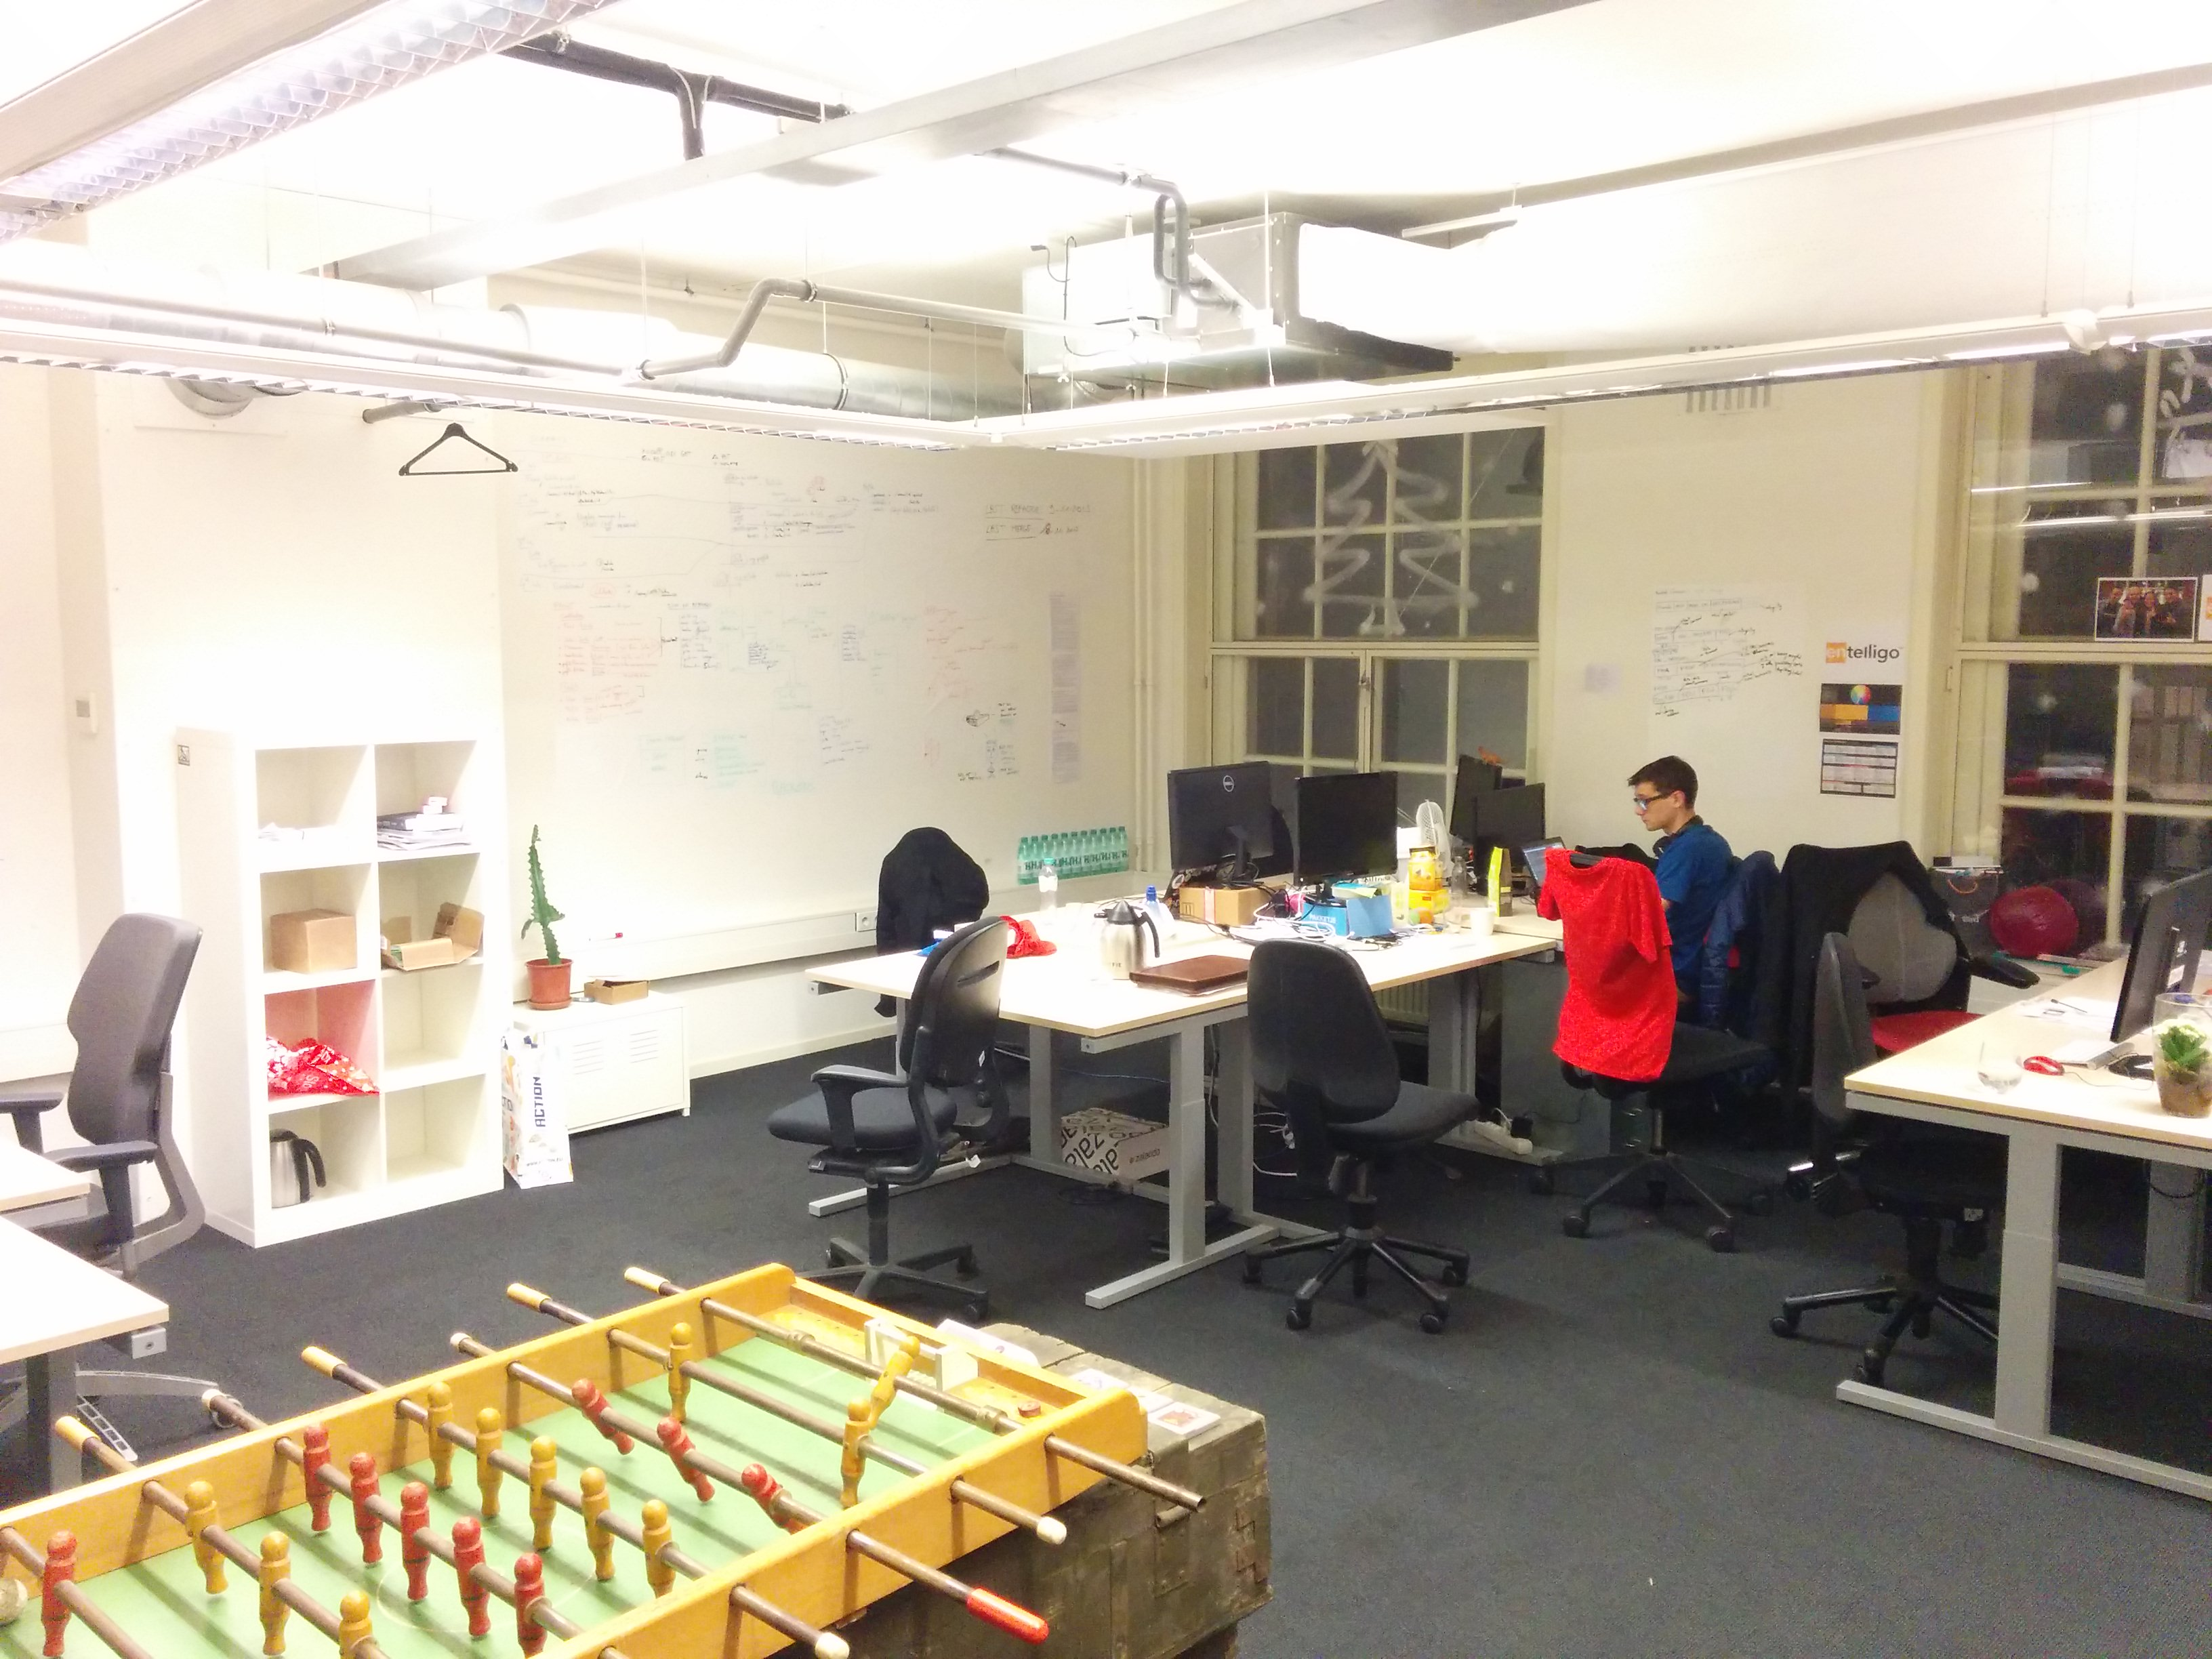
\includegraphics[width=0.75\textwidth]{images/office.jpg}
   \caption[Our office]{Our office}
\end{figure}

The Smiths has its office located at Herengracht 182, in Amsterdam. It is in the very city center, close to everything. We were in an incubator called \textbf{\href{http://www.rockstart.com/}{Rockstart}} whose mottos are "\textit{Step Forward. Start.}" and "\textit{We love startups}". Basically, they provide startups with as many desks as they need, in one of the four floors, with free coffee and tea. In parallel, they prepare everything for lunch at a reasonable price. Moreover, every startup can book a huge old ballroom for special events, most of the time for free.

\medskip

It is a very nice place for startups to prosper, so inspiring, full of young people, mostly developers. The atmosphere is really favorable to innovation, there is always someone challenging your ideas. What is more, we would often organize some crazy foosball competitions after lunch.

\subsection{Influence}

The Smiths has proven its clients a great ability to ship good mobile applications, highly scalable, and more importantly, with a good evolvability. Quite surprisingly, within a few months, The Smiths caught on with the Titanium community, thanks to a huge commitment.

\medskip

Every month, the Smiths were given the mission to organize the official Titanium meeting events. With an average of twenty attendees, there was usually three or four speakers, giving talks about mobile development with Titanium or any other related topic. The meetups were always sponsored by Appcelerator, the company behind Titanium, providing everyone with food and drinks.

\medskip

The company's commitment (and especially Matthias') to giving away open source modules, plugins or widgets allowed us to get praised sometimes.

\section{Titanium}

\begin{figure}[!h]
   \centering
\includegraphics[width=0.4\textwidth]{images/titanium.png}
   \caption{Titanium SDK}
\end{figure}

As I said earlier, everyone at the Smiths is dedicated to developing mobile applications with Titanium. So, let's dive into Titanium and look under the hood.

\subsection{Concept}

Titanium is an open-source framework\footnote{More or less a foundation, a structure or a platform for developers to build software programs. The code of a framework generally offers classes and functions that can be either reused of changed by user-written code. It is quite similar to an API (frameworks technically contains API(s)). "Framework" is a generic term that can basically define a lot for things.}/SDK, powered by Appcelerator, that allows developers to create and ship mobile apps very quickly, for both Android and iOS (and Windows Mobile), or create responsive web pages -- and all of this with the same codebase, written in JavaScript. It was firstly introduced in late 2008.

\medskip

Out of the box, Titanium does not impose nor recommend any particular project structure. The lack of best practices regarding project structures was, by the way, one of the biggest downsides in Titanium for years.

\medskip

However, since 2012, developers can also add a MVC-based\footnote{\textit{Model View Controller}, a popular architecture in software} framework on top of Titanium called Alloy, to bring a better architecture to their apps. It was designed to "\textit{rapidly develop quality Titanium applications}". To support the MVC architecture, the creators of Alloy also added \href{http://backbonejs.org/}{Backbone.js} and \href{http://underscorejs.org/}{Underscore.js}, which are JavaScript libraries, respectively providing Titanium with models (plus collections and events) and functional helpers.

\medskip

Basically, an accepted definition of working with Titanium could be

\begin{quote}
\textit{Simply write JavaScript code, Titanium will turn it into native code for each platform.}---Romain Pellerin
\end{quote}
In fact, not exactly. The JavaScript code is evaluated at runtime\footnote{When the mobile app is running}. Actually, what is in native code is the Titanium API\footnote{\textit{Application Programming Interface}, a set of routines, protocols and tools exposed to API consumers, to interact with a remote database or software for example. It is a level of abstraction.}, which acts as a "bridge" or "proxy" between our JavaScript code and the system calls (made in native code, depending on the platform, either in Java or Objective-C/Swift).

\subsection{Appcelerator}

Appcelerator is the company behind Titanium. Its core mission is obviously to support the development of Titanium, but not only. As Titanium is open-source, they mostly developed their business model thanks to other services. More and more, they tend to target enterprises instead of independent developers to generate revenue. As examples, their most successful products include real-time analytics, cloud services, and push notifications\footnote{For more information about their range of products, see \href{http://www.appcelerator.com/product/}{www.appcelerator.com/product/}}. They also provide their own IDE\footnote{\textit{Integrated Development Environment}, or more simply, a text editor linked to a compiler, with built-in tools like a linter, an embedded console, a source management system (Git or SVN, mainly), etc.} based on Eclipse, for free, as an alternative to the CLI\footnote{\textit{Command Line Interface}}.

\subsection{Alloy}

As exposed above, Appcelerator introduced in 2012 a new framework called Alloy. Basically, it is just a Titanium plugin (plugins will be quickly explained right below). This means that it is a piece of code run in the very first step of compilation. Briefly, what it brings are:

\begin{itemize}
  \item XML support to write and define views
  \item A new file format, \textbf{.tss}, a cousin of CSS, to declare styles and themes for views
  \item A new structure for Titanium projects, to better organize files under a relevant architecture
  \item A handful of global functions and variables aimed at easing simple tasks and objects storing, likewise a configuration file complementary to the original one provided by Titanium
  \item Two powerful JavaScript libraries: Backbone and Underscore (they respectively bring models and helpers)
\end{itemize}

Here is a new structure brought by Alloy, in the root directory \lstinline{app/}:

\begin{figure}[!h]
   \centering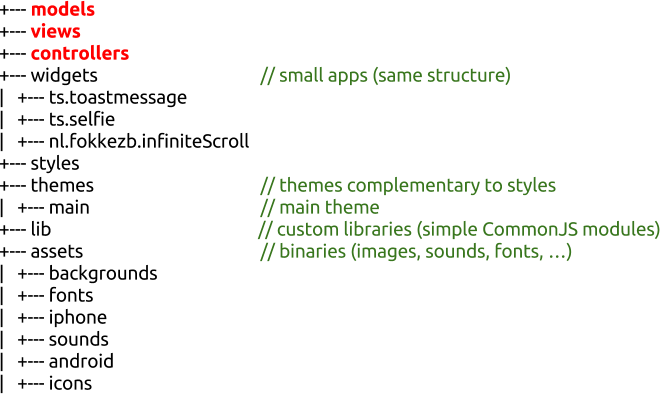
\includegraphics[width=0.8\textwidth]{images/Alloy.png}
   \caption[Alloy structure]{Alloy structure\\\textit{The widgets here are given as examples}}
\end{figure}

\subsubsection{How it works}

The way Alloy works is pretty simple and adds a lot of logic. There is a file at the root of \lstinline{app/}, called \lstinline{alloy.js}. It is the first file executed when the app is being launched. Then, Alloy runs the default controller located at \lstinline{controllers/index.js}. It also loads a default view if existing (\lstinline{views/index.js}) and it applies styles to that view (if existing as well, from \lstinline{styles/index.js} or from \lstinline{themes/}). Then, developers can start any other controller from an opened one, just by calling a built-in function of Alloy. The app will automatically try to launch the corresponding view and apply the corresponding styling (always according to the controller's name).

\subsection{Modules, widgets and plugins}

In spite of the fact that Titanium covers most of the native features available on both Android and iOS, it can not be 100\% up-to-date, considering new versions of Android and iOS are generally coming out once a year. Thus, they had to provide a way for developers to satisfy all their needs regarding cutting-edge features. Consequently, they "invented" modules.\\
Modules are one of the many strengths of Titanium. Modules are mostly written in native code (either Java for Android or Objective-C for iOS). They allow developers to add missing features to Titanium. Just like the official Titanium API, modules offer missing JavaScript APIs to Titanium developers. Many are available on the Web, either created by Appcelerator or independent developers.\\
For example, at some point I was looking for a way to add in-app purchases in an app. On Android, this feature is provided by the Google Services, which are not part of core Android -- it is a third-party app. Consequently, Titanium cannot bring it either, as it might be updated at any time by Google, and is not correlated to Android itself. In such a situation, modules are what I needed.

\medskip

On the other hand, widgets are small pieces of JavaScript code whose purpose is to add reusable components to an app, such as views, specific models or mere convenient functions. In simple words, one could see widgets as a Titanium app taken apart into smaller bits. Those bits can be made reusable, and then shared on the Web among the Titanium community. This way, one does not have to reinvent the wheel and can reuse other people's work. Widgets are brought by Alloy and have their own views, controllers, styles and assets.\\
As examples, there are widgets that bring helpers for API calls, some others bring views (a chat view for instance, with the input field and the list of messages), and so forth.\\
Widgets are much simpler pieces of code than modules and only written in JavaScript (and XML/TSS if they add view(s) and styling to them). They are minimalist Titanium apps with roughly the same file structure.

\medskip

Finally, Titanium also support plugins. Alloy is a concrete example of a plugin. I will not explain any further but in short, it is code being executed at the beginning of the compilation. Matthias, my colleague, created a plugin that transpiled\footnote{Transpiling is "taking source code written in one language and transforming into another language that has a similar level of abstraction". Source: \href{https://www.stevefenton.co.uk/2012/11/compiling-vs-transpiling/}{www.stevefenton.co.uk/2012/11/compiling-vs-transpiling/}} code written in ES6\footnote{ECMAScript 6, a.k.a ECMAScript 2015, is the latest JavaScript Specification, still not supported by Titanium and most web browsers} into ES5 thanks to Babel (a compiler whose only job is to transpile ES6 code into ES5). That process was automatically run right before the compilation, thanks to some tuning made with Titanium. He made it available\footnote{\href{https://www.npmjs.com/package/ti.es6}{www.npmjs.com/package/ti.es6}} to everyone and encountered a quite huge success quickly.

\subsection{Motivation to use Titanium}

Quite simply, the Smiths already had experience with Titanium in their previous startup (WappZapp). They could have decided to get back to native development or try another cross-platform tool but instead they decided to keep on with Titanium. Why? Merely because it is a robust SDK quite reliable, under intense development with an increasing community. Furthermore, it would allow the company to save money (one JavaScript developer is more easily findable and often cheaper than either a developer able to develop on both Android and iOS, or two distinct developers).

\section{My mission}

When I accepted the internship offer, in late Spring 2015, I got assigned one particular mission. The Smiths had just come to an agreement with a client for a new project and I would be responsible for the whole project, from the specifications to delivering the final product.

\medskip

After this first mission (abruptly aborted, but that will come later), I was reoriented to an internal project called KopenVerkopen, which is an app for selling items (like eBay). I also worked on another project for a different client, mostly in January 2016. For these purposes, I had to develop some Titanium widgets that the Smiths would reuse later.

\medskip

Aside my main missions, I have been trying to design a robust and efficient workflow. By workflow, I mean a tested and approved process for developing a software project. From the source code management, to shipping the product, including some automation, automated testing, and so on.\\
In the meantime, I also worked on APIs, trying to define a standard we would follow for each project, simple to use, evolvable and which takes advantage of all the strengths of the protocol HTTP.\\
Those two aside topics (APIs and workflow) will be treated in the next chapters to ease the overall understanding of this report. Then, the three projects will come in the remaining chapters.